\documentclass[crop,tikz]{standalone}
\usetikzlibrary{backgrounds}
\colorlet{blue}{cyan}
\tikzset{
  inverted/.style = {
    color=white,
    background rectangle/.style={fill},
    show background rectangle
  }
}

\tikzset{>=latex}

\begin{document}
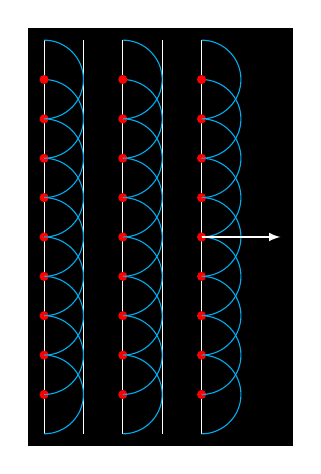
\begin{tikzpicture}[inverted,inverted]
  \foreach \X in {0,0.5,1,1.5,2} { \draw (\X,0) -- +(0,5); }
  \foreach \X in {0,1,2} {%
    \foreach \Y in {0.5,1,...,4.5} {%
      \draw[blue] (\X,\Y)+(-90:0.5) arc (-90:90:0.5);
      \draw[fill,red] (\X,\Y) circle (0.05);
    }
  }
  \draw[->] (2,2.5) -- +(1,0);
\end{tikzpicture}
\end{document}
